\documentclass[]{book}
\usepackage{lmodern}
\usepackage{amssymb,amsmath}
\usepackage{ifxetex,ifluatex}
\usepackage{fixltx2e} % provides \textsubscript
\ifnum 0\ifxetex 1\fi\ifluatex 1\fi=0 % if pdftex
  \usepackage[T1]{fontenc}
  \usepackage[utf8]{inputenc}
\else % if luatex or xelatex
  \ifxetex
    \usepackage{mathspec}
  \else
    \usepackage{fontspec}
  \fi
  \defaultfontfeatures{Ligatures=TeX,Scale=MatchLowercase}
\fi
% use upquote if available, for straight quotes in verbatim environments
\IfFileExists{upquote.sty}{\usepackage{upquote}}{}
% use microtype if available
\IfFileExists{microtype.sty}{%
\usepackage{microtype}
\UseMicrotypeSet[protrusion]{basicmath} % disable protrusion for tt fonts
}{}
\usepackage[margin=1in]{geometry}
\usepackage{hyperref}
\hypersetup{unicode=true,
            pdftitle={Statistics 1},
            pdfborder={0 0 0},
            breaklinks=true}
\urlstyle{same}  % don't use monospace font for urls
\usepackage{color}
\usepackage{fancyvrb}
\newcommand{\VerbBar}{|}
\newcommand{\VERB}{\Verb[commandchars=\\\{\}]}
\DefineVerbatimEnvironment{Highlighting}{Verbatim}{commandchars=\\\{\}}
% Add ',fontsize=\small' for more characters per line
\usepackage{framed}
\definecolor{shadecolor}{RGB}{248,248,248}
\newenvironment{Shaded}{\begin{snugshade}}{\end{snugshade}}
\newcommand{\KeywordTok}[1]{\textcolor[rgb]{0.13,0.29,0.53}{\textbf{#1}}}
\newcommand{\DataTypeTok}[1]{\textcolor[rgb]{0.13,0.29,0.53}{#1}}
\newcommand{\DecValTok}[1]{\textcolor[rgb]{0.00,0.00,0.81}{#1}}
\newcommand{\BaseNTok}[1]{\textcolor[rgb]{0.00,0.00,0.81}{#1}}
\newcommand{\FloatTok}[1]{\textcolor[rgb]{0.00,0.00,0.81}{#1}}
\newcommand{\ConstantTok}[1]{\textcolor[rgb]{0.00,0.00,0.00}{#1}}
\newcommand{\CharTok}[1]{\textcolor[rgb]{0.31,0.60,0.02}{#1}}
\newcommand{\SpecialCharTok}[1]{\textcolor[rgb]{0.00,0.00,0.00}{#1}}
\newcommand{\StringTok}[1]{\textcolor[rgb]{0.31,0.60,0.02}{#1}}
\newcommand{\VerbatimStringTok}[1]{\textcolor[rgb]{0.31,0.60,0.02}{#1}}
\newcommand{\SpecialStringTok}[1]{\textcolor[rgb]{0.31,0.60,0.02}{#1}}
\newcommand{\ImportTok}[1]{#1}
\newcommand{\CommentTok}[1]{\textcolor[rgb]{0.56,0.35,0.01}{\textit{#1}}}
\newcommand{\DocumentationTok}[1]{\textcolor[rgb]{0.56,0.35,0.01}{\textbf{\textit{#1}}}}
\newcommand{\AnnotationTok}[1]{\textcolor[rgb]{0.56,0.35,0.01}{\textbf{\textit{#1}}}}
\newcommand{\CommentVarTok}[1]{\textcolor[rgb]{0.56,0.35,0.01}{\textbf{\textit{#1}}}}
\newcommand{\OtherTok}[1]{\textcolor[rgb]{0.56,0.35,0.01}{#1}}
\newcommand{\FunctionTok}[1]{\textcolor[rgb]{0.00,0.00,0.00}{#1}}
\newcommand{\VariableTok}[1]{\textcolor[rgb]{0.00,0.00,0.00}{#1}}
\newcommand{\ControlFlowTok}[1]{\textcolor[rgb]{0.13,0.29,0.53}{\textbf{#1}}}
\newcommand{\OperatorTok}[1]{\textcolor[rgb]{0.81,0.36,0.00}{\textbf{#1}}}
\newcommand{\BuiltInTok}[1]{#1}
\newcommand{\ExtensionTok}[1]{#1}
\newcommand{\PreprocessorTok}[1]{\textcolor[rgb]{0.56,0.35,0.01}{\textit{#1}}}
\newcommand{\AttributeTok}[1]{\textcolor[rgb]{0.77,0.63,0.00}{#1}}
\newcommand{\RegionMarkerTok}[1]{#1}
\newcommand{\InformationTok}[1]{\textcolor[rgb]{0.56,0.35,0.01}{\textbf{\textit{#1}}}}
\newcommand{\WarningTok}[1]{\textcolor[rgb]{0.56,0.35,0.01}{\textbf{\textit{#1}}}}
\newcommand{\AlertTok}[1]{\textcolor[rgb]{0.94,0.16,0.16}{#1}}
\newcommand{\ErrorTok}[1]{\textcolor[rgb]{0.64,0.00,0.00}{\textbf{#1}}}
\newcommand{\NormalTok}[1]{#1}
\usepackage{longtable,booktabs}
\usepackage{graphicx,grffile}
\makeatletter
\def\maxwidth{\ifdim\Gin@nat@width>\linewidth\linewidth\else\Gin@nat@width\fi}
\def\maxheight{\ifdim\Gin@nat@height>\textheight\textheight\else\Gin@nat@height\fi}
\makeatother
% Scale images if necessary, so that they will not overflow the page
% margins by default, and it is still possible to overwrite the defaults
% using explicit options in \includegraphics[width, height, ...]{}
\setkeys{Gin}{width=\maxwidth,height=\maxheight,keepaspectratio}
\IfFileExists{parskip.sty}{%
\usepackage{parskip}
}{% else
\setlength{\parindent}{0pt}
\setlength{\parskip}{6pt plus 2pt minus 1pt}
}
\setlength{\emergencystretch}{3em}  % prevent overfull lines
\providecommand{\tightlist}{%
  \setlength{\itemsep}{0pt}\setlength{\parskip}{0pt}}
\setcounter{secnumdepth}{5}
% Redefines (sub)paragraphs to behave more like sections
\ifx\paragraph\undefined\else
\let\oldparagraph\paragraph
\renewcommand{\paragraph}[1]{\oldparagraph{#1}\mbox{}}
\fi
\ifx\subparagraph\undefined\else
\let\oldsubparagraph\subparagraph
\renewcommand{\subparagraph}[1]{\oldsubparagraph{#1}\mbox{}}
\fi

%%% Use protect on footnotes to avoid problems with footnotes in titles
\let\rmarkdownfootnote\footnote%
\def\footnote{\protect\rmarkdownfootnote}

%%% Change title format to be more compact
\usepackage{titling}

% Create subtitle command for use in maketitle
\newcommand{\subtitle}[1]{
  \posttitle{
    \begin{center}\large#1\end{center}
    }
}

\setlength{\droptitle}{-2em}
  \title{Statistics 1}
  \pretitle{\vspace{\droptitle}\centering\huge}
  \posttitle{\par}
  \author{}
  \preauthor{}\postauthor{}
  \date{}
  \predate{}\postdate{}


\usepackage{amsthm}
\newtheorem{theorem}{Theorem}[chapter]
\newtheorem{lemma}{Lemma}[chapter]
\theoremstyle{definition}
\newtheorem{definition}{Definition}[chapter]
\newtheorem{corollary}{Corollary}[chapter]
\newtheorem{proposition}{Proposition}[chapter]
\theoremstyle{definition}
\newtheorem{example}{Example}[chapter]
\theoremstyle{definition}
\newtheorem{exercise}{Exercise}[chapter]
\theoremstyle{remark}
\newtheorem*{remark}{Remark}
\newtheorem*{solution}{Solution}
\begin{document}
\maketitle

{
\setcounter{tocdepth}{1}
\tableofcontents
}
\chapter*{About this course}\label{about-this-course}
\addcontentsline{toc}{chapter}{About this course}

This course is an introduction to data science. We have three primary
aims. First, to introduce you to the logic of quantitative research
design. Second, to familiarise you with statistical models that
scientists and policy-makers use to answer social science questions.
Third, to help you acquire the necessary skills to conduct your own
quantitative research projects. No prior statistical knowledge is
assumed. We will use the statistical software R and RStudio on top.

\begin{center}\rule{0.5\linewidth}{\linethickness}\end{center}

Syllabus

Moodle

Piazza

\chapter{Introduction: Measurement, Central Tendency, Dispersion,
Validity,
Reliability}\label{introduction-measurement-central-tendency-dispersion-validity-reliability}

\section{Seminar}\label{seminar}

In this seminar session, we introduce working with R. We illustrate some
basic functionality and help you familiarise yourself with the look and
feel of RStudio. Measures of central tendency and dispersion are easy to
calculate in R. We focus on introducing the logic of R first and then
describe how central tendency and dispersion are calculated in the end
of the seminar.

\subsection{Getting Started}\label{getting-started}

Install R and RStudio on your computer by downloading them from the
following sources:

\begin{itemize}
\tightlist
\item
  Download R from \href{https://cran.r-project.org}{The Comprehensive R
  Archive Network (CRAN)}
\item
  Download RStudio from \href{https://www.rstudio.com}{RStudio.com}
\end{itemize}

\subsection{RStudio}\label{rstudio}

Let's get acquainted with R. When you start RStudio for the first time,
you'll see three panes:

\begin{figure}
\centering
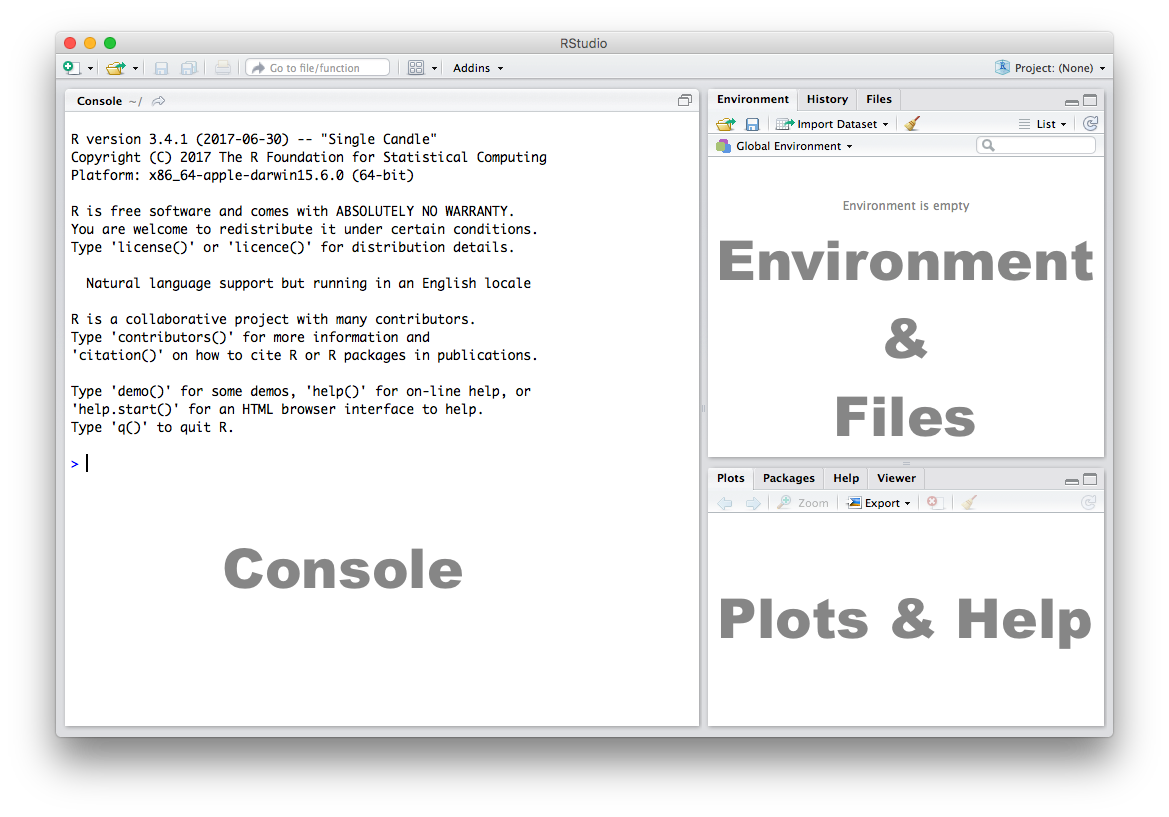
\includegraphics{./img/rstudio_default.png}
\caption{}
\end{figure}

\subsection{Console}\label{console}

The Console in RStudio is the simplest way to interact with R. You can
type some code at the Console and when you press ENTER, R will run that
code. Depending on what you type, you may see some output in the Console
or if you make a mistake, you may get a warning or an error message.

Let's familiarize ourselves with the console by using R as a simple
calculator:

\begin{Shaded}
\begin{Highlighting}[]
\DecValTok{2} \OperatorTok{+}\StringTok{ }\DecValTok{4}
\end{Highlighting}
\end{Shaded}

\begin{verbatim}
[1] 6
\end{verbatim}

Now that we know how to use the \texttt{+} sign for addition, let's try
some other mathematical operations such as subtraction (\texttt{-}),
multiplication (\texttt{*}), and division (\texttt{/}).

\begin{Shaded}
\begin{Highlighting}[]
\DecValTok{10} \OperatorTok{-}\StringTok{ }\DecValTok{4}
\end{Highlighting}
\end{Shaded}

\begin{verbatim}
[1] 6
\end{verbatim}

\begin{Shaded}
\begin{Highlighting}[]
\DecValTok{5} \OperatorTok{*}\StringTok{ }\DecValTok{3}
\end{Highlighting}
\end{Shaded}

\begin{verbatim}
[1] 15
\end{verbatim}

\begin{Shaded}
\begin{Highlighting}[]
\DecValTok{7} \OperatorTok{/}\StringTok{ }\DecValTok{2}
\end{Highlighting}
\end{Shaded}

\begin{verbatim}
[1] 3.5
\end{verbatim}

\begin{longtable}[]{@{}ll@{}}
\toprule
\begin{minipage}[t]{0.69\columnwidth}\raggedright\strut
You can use the cursor or arrow keys on your keyboard to edit your code
at the console:- Use the UP and DOWN keys to re-run something without
typing it again- Use the LEFT and RIGHT keys to edit\strut
\end{minipage} & \begin{minipage}[t]{0.25\columnwidth}\raggedright\strut
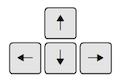
\includegraphics{./img/rstudio_cursorkeys.png}\strut
\end{minipage}\tabularnewline
\bottomrule
\end{longtable}

Take a few minutes to play around at the console and try different
things out. Don't worry if you make a mistake, you can't break anything
easily!

\subsection{Functions}\label{functions}

Functions are a set of instructions that carry out a specific task.
Functions often require some input and generate some output. For
example, instead of using the \texttt{+} operator for addition, we can
use the \texttt{sum} function to add two or more numbers.

\begin{Shaded}
\begin{Highlighting}[]
\KeywordTok{sum}\NormalTok{(}\DecValTok{1}\NormalTok{, }\DecValTok{4}\NormalTok{, }\DecValTok{10}\NormalTok{)}
\end{Highlighting}
\end{Shaded}

\begin{verbatim}
[1] 15
\end{verbatim}

In the example above, \texttt{1,\ 4,\ 10} are the inputs and 15 is the
output. A function always requires the use of parenthesis or round
brackets \texttt{()}. Inputs to the function are called
\textbf{arguments} and go inside the brackets. The output of a function
is displayed on the screen but we can also have the option of saving the
result of the output. More on this later.

\subsection{Getting Help}\label{getting-help}

Another useful function in R is \texttt{help} which we can use to
display online documentation. For example, if we wanted to know how to
use the \texttt{sum} function, we could type \texttt{help(sum)} and look
at the online documentation.

\begin{Shaded}
\begin{Highlighting}[]
\KeywordTok{help}\NormalTok{(sum)}
\end{Highlighting}
\end{Shaded}

The question mark \texttt{?} can also be used as a shortcut to access
online help.

\begin{Shaded}
\begin{Highlighting}[]
\NormalTok{?sum}
\end{Highlighting}
\end{Shaded}

\begin{figure}
\centering
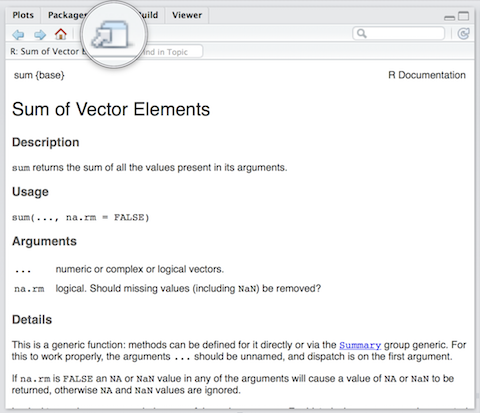
\includegraphics{./img/rstudio_help.png}
\caption{}
\end{figure}

Use the toolbar button shown in the picture above to expand and display
the help in a new window.

Help pages for functions in R follow a consistent layout generally
include these sections:

\begin{longtable}[]{@{}ll@{}}
\toprule
Description & A brief description of the function\tabularnewline
Usage & The complete syntax or grammar including all arguments
(inputs)\tabularnewline
Arguments & Explanation of each argument\tabularnewline
Details & Any relevant details about the function and its
arguments\tabularnewline
Value & The output value of the function\tabularnewline
Examples & Example of how to use the function\tabularnewline
\bottomrule
\end{longtable}

\subsection{The Assignment Operator}\label{the-assignment-operator}

Now we know how to provide inputs to a function using parenthesis or
round brackets \texttt{()}, but what about the output of a function?

We use the assignment operator \textbf{\texttt{\textless{}-}} for
creating or updating objects. If we wanted to save the result of adding
\texttt{sum(1,\ 4,\ 10)}, we would do the following:

\begin{Shaded}
\begin{Highlighting}[]
\NormalTok{myresult <-}\StringTok{ }\KeywordTok{sum}\NormalTok{(}\DecValTok{1}\NormalTok{, }\DecValTok{4}\NormalTok{, }\DecValTok{10}\NormalTok{)}
\end{Highlighting}
\end{Shaded}

The line above creates a new object called \texttt{myresult} in our
environment and saves the result of the \texttt{sum(1,\ 4,\ 10)} in it.
To see what's in \texttt{myresult}, just type it at the console:

\begin{Shaded}
\begin{Highlighting}[]
\NormalTok{myresult}
\end{Highlighting}
\end{Shaded}

\begin{verbatim}
[1] 15
\end{verbatim}

Take a look at the \textbf{Environment} pane in RStudio and you'll see
\texttt{myresult} there.

\begin{figure}
\centering
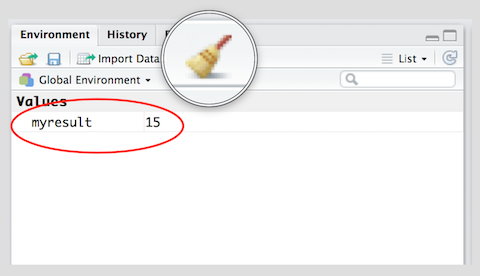
\includegraphics{./img/rstudio_env.png}
\caption{}
\end{figure}

To delete all objects from the environment, you can use the
\textbf{broom} button as shown in the picture above.

We called our object \texttt{myresult} but we can call it anything as
long as we follow a few simple rules. Object names can contain upper or
lower case letters (\texttt{A-Z}, \texttt{a-z}), numbers (\texttt{0-9}),
underscores (\texttt{\_}) or a dot (\texttt{.}) but all object names
must start with a letter. Choose names that are descriptive and easy to
type.

\begin{longtable}[]{@{}ll@{}}
\toprule
Good Object Names & Bad Object Names\tabularnewline
\midrule
\endhead
result & a\tabularnewline
myresult & x1\tabularnewline
my.result & this.name.is.just.too.long\tabularnewline
my\_result &\tabularnewline
data1 &\tabularnewline
\bottomrule
\end{longtable}

\subsection{Sequences}\label{sequences}

We often need to create sequences when manipulating data. For instance,
you might want to perform an operation on the first 10 rows of a dataset
so we need a way to select the range we're interested in.

There are two ways to create a sequence. Let's try to create a sequence
of numbers from 1 to 10 using the two methods:

\begin{enumerate}
\def\labelenumi{\arabic{enumi}.}
\tightlist
\item
  Using the colon \texttt{:} operator. If you're familiar with
  spreadsheets then you might've already used \texttt{:} to select
  cells, for example \texttt{A1:A20}. In R, you can use the \texttt{:}
  to create a sequence in a similar fashion:
\end{enumerate}

\begin{Shaded}
\begin{Highlighting}[]
\DecValTok{1}\OperatorTok{:}\DecValTok{10}
\end{Highlighting}
\end{Shaded}

\begin{verbatim}
 [1]  1  2  3  4  5  6  7  8  9 10
\end{verbatim}

\begin{enumerate}
\def\labelenumi{\arabic{enumi}.}
\tightlist
\item
  Using the \texttt{seq} function we get the exact same result:
\end{enumerate}

\begin{Shaded}
\begin{Highlighting}[]
\KeywordTok{seq}\NormalTok{(}\DataTypeTok{from =} \DecValTok{1}\NormalTok{, }\DataTypeTok{to =} \DecValTok{10}\NormalTok{)}
\end{Highlighting}
\end{Shaded}

\begin{verbatim}
 [1]  1  2  3  4  5  6  7  8  9 10
\end{verbatim}

The \texttt{seq} function has a number of options which control how the
sequence is generated. For example to create a sequence from 0 to 100 in
increments of \texttt{5}, we can use the optional \texttt{by} argument.
Notice how we wrote \texttt{by\ =\ 5} as the third argument. It is a
common practice to specify the name of argument when the argument is
optional. The arguments \texttt{from} and \texttt{to} are not optional,
se we can write \texttt{seq(0,\ 100,\ by\ =\ 5)} instead of
\texttt{seq(from\ =\ 0,\ to\ =\ 100,\ by\ =\ 5)}. Both, are valid ways
of achieving the same outcome. You can code whichever way you like. We
recommend to write code such that you make it easy for your future self
and others to read and understand the code.

\begin{Shaded}
\begin{Highlighting}[]
\KeywordTok{seq}\NormalTok{(}\DataTypeTok{from =} \DecValTok{0}\NormalTok{, }\DataTypeTok{to =} \DecValTok{100}\NormalTok{, }\DataTypeTok{by =} \DecValTok{5}\NormalTok{)}
\end{Highlighting}
\end{Shaded}

\begin{verbatim}
 [1]   0   5  10  15  20  25  30  35  40  45  50  55  60  65  70  75  80
[18]  85  90  95 100
\end{verbatim}

Another common use of the \texttt{seq} function is to create a sequence
of a specific length. Here, we create a sequence from 0 to 100 with
length 9, i.e., the result is a vector with 9 elements.

\begin{Shaded}
\begin{Highlighting}[]
\KeywordTok{seq}\NormalTok{(}\DataTypeTok{from =} \DecValTok{0}\NormalTok{, }\DataTypeTok{to =} \DecValTok{100}\NormalTok{, }\DataTypeTok{length.out =}  \DecValTok{9}\NormalTok{)}
\end{Highlighting}
\end{Shaded}

\begin{verbatim}
[1]   0.0  12.5  25.0  37.5  50.0  62.5  75.0  87.5 100.0
\end{verbatim}

Now it's your turn:

\begin{itemize}
\tightlist
\item
  Create a sequence of \textbf{odd} numbers between 0 and 100 and save
  it in an object called \texttt{odd\_numbers}
\end{itemize}

\begin{Shaded}
\begin{Highlighting}[]
\NormalTok{odd_numbers <-}\StringTok{ }\KeywordTok{seq}\NormalTok{(}\DecValTok{1}\NormalTok{, }\DecValTok{100}\NormalTok{, }\DecValTok{2}\NormalTok{)}
\end{Highlighting}
\end{Shaded}

\begin{itemize}
\tightlist
\item
  Next, display \texttt{odd\_numbers} on the console to verify that you
  did it correctly
\end{itemize}

\begin{Shaded}
\begin{Highlighting}[]
\NormalTok{odd_numbers}
\end{Highlighting}
\end{Shaded}

\begin{verbatim}
 [1]  1  3  5  7  9 11 13 15 17 19 21 23 25 27 29 31 33 35 37 39 41 43 45
[24] 47 49 51 53 55 57 59 61 63 65 67 69 71 73 75 77 79 81 83 85 87 89 91
[47] 93 95 97 99
\end{verbatim}

\begin{itemize}
\item
  What do the numbers in square brackets \texttt{{[}\ {]}} mean? Look at
  the number of values displayed in each line to find out the answer.
\item
  Use the \texttt{length} function to find out how many values are in
  the object \texttt{odd\_numbers}.

  \begin{itemize}
  \tightlist
  \item
    HINT: Try \texttt{help(length)} and look at the examples section at
    the end of the help screen.
  \end{itemize}
\end{itemize}

\begin{Shaded}
\begin{Highlighting}[]
\KeywordTok{length}\NormalTok{(odd_numbers)}
\end{Highlighting}
\end{Shaded}

\begin{verbatim}
[1] 50
\end{verbatim}

\subsection{Scripts}\label{scripts}

The Console is great for simple tasks but if you're working on a project
you would mostly likely want to save your work in some sort of a
document or a file. Scripts in R are just plain text files that contain
R code. You can edit a script just like you would edit a file in any
word processing or note-taking application.

Create a new script using the menu or the toolbar button as shown below.

\begin{figure}
\centering
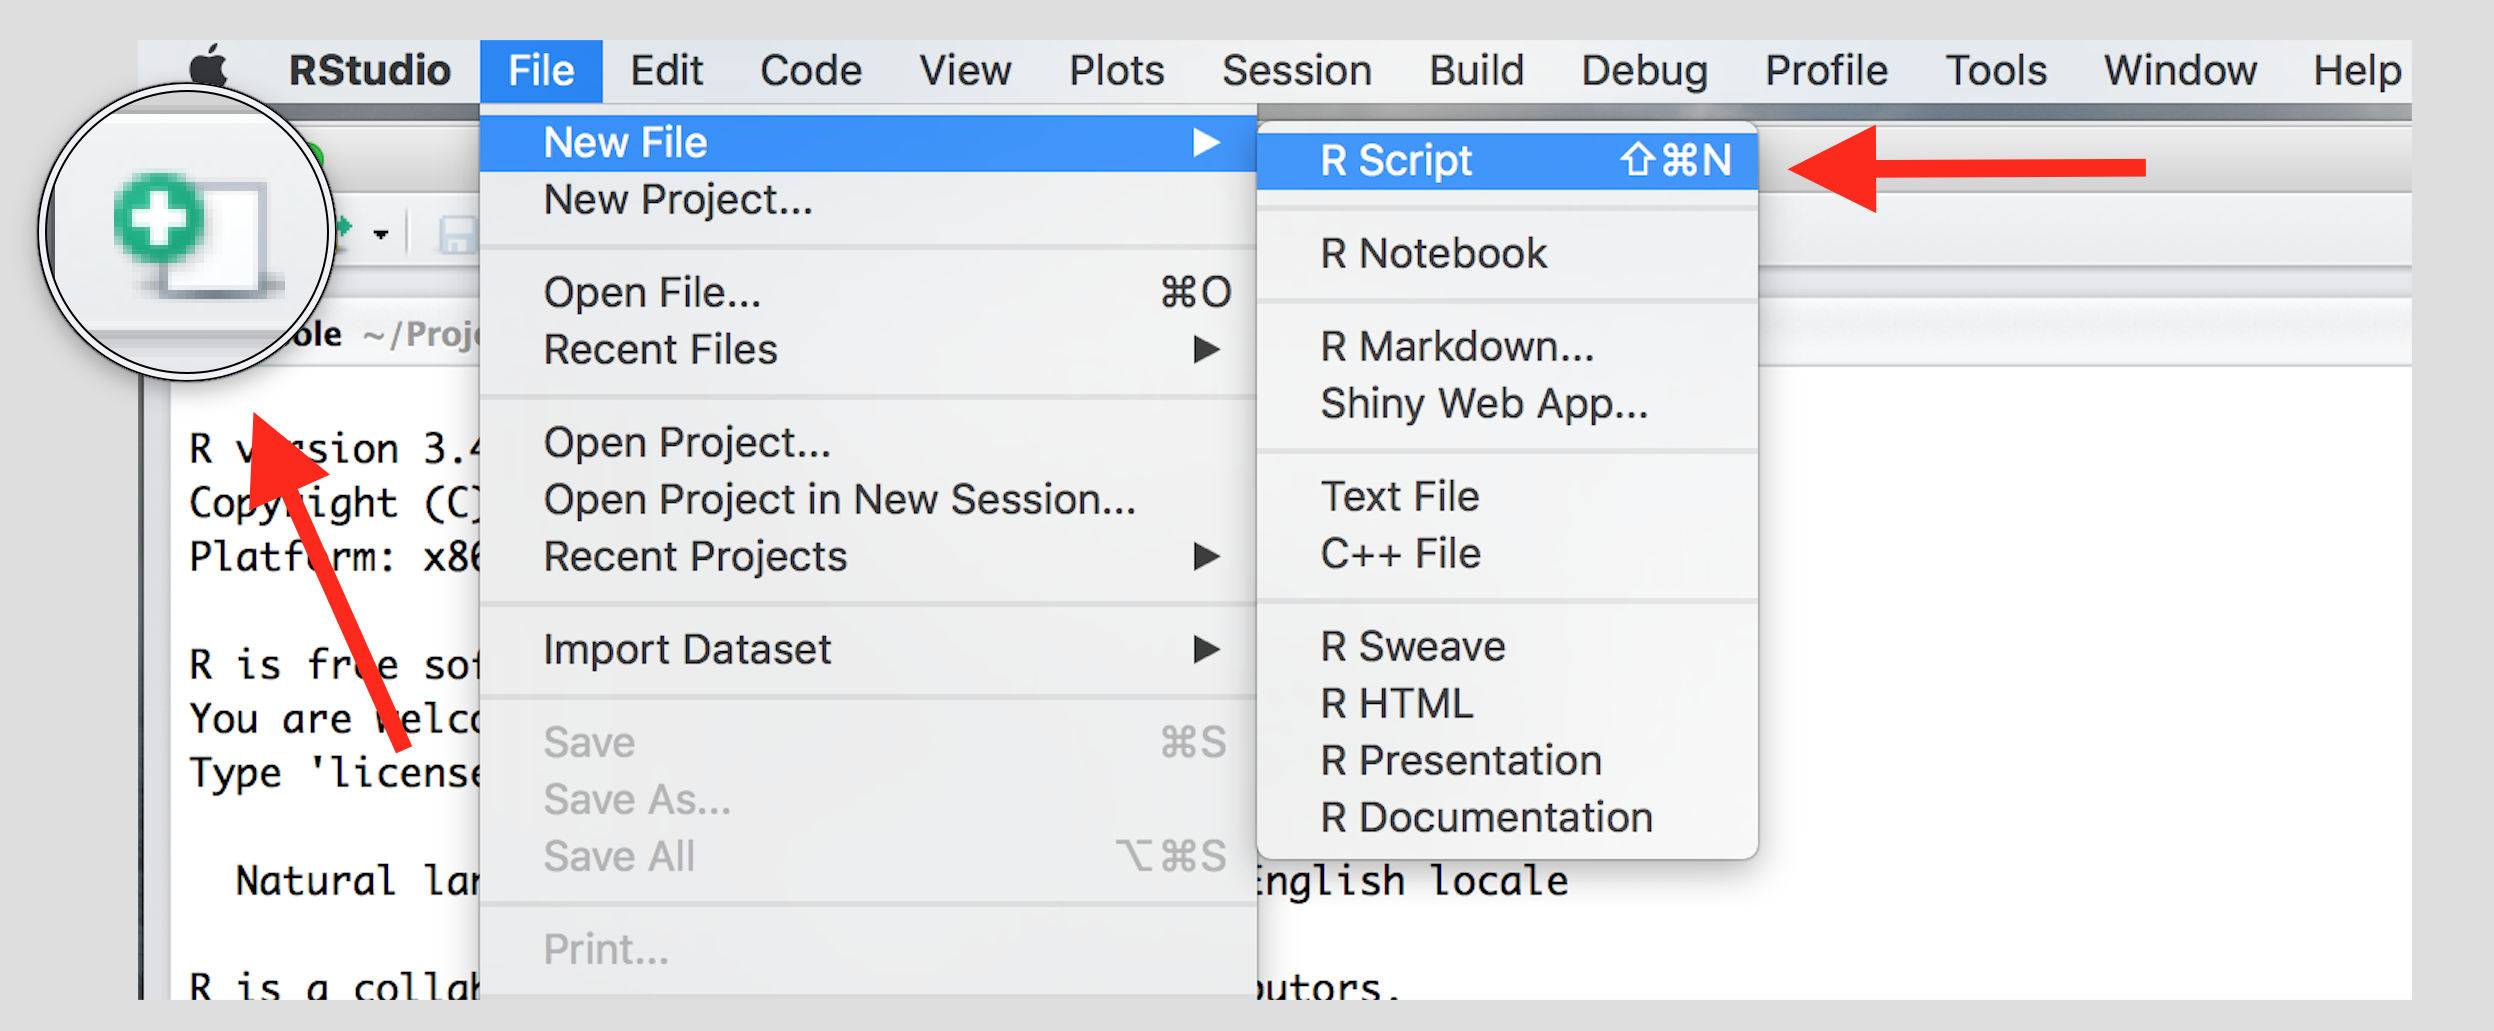
\includegraphics{./img/rstudio_newfile.png}
\caption{}
\end{figure}

Once you've created a script, it is generally a good idea to give it a
meaningful name and save it immediately. For our first session save your
script as \textbf{seminar1.R}

\begin{longtable}[]{@{}ll@{}}
\toprule
\begin{minipage}[t]{0.52\columnwidth}\raggedright\strut
Familiarize yourself with the script window in RStudio, and especially
the two buttons labeled \textbf{Run} and \textbf{Source}\strut
\end{minipage} & \begin{minipage}[t]{0.42\columnwidth}\raggedright\strut
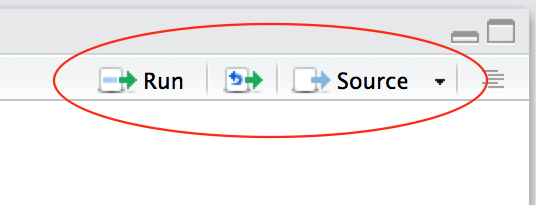
\includegraphics{./img/rstudio_script.png}\strut
\end{minipage}\tabularnewline
\bottomrule
\end{longtable}

There are a few different ways to run your code from a script.

\begin{longtable}[]{@{}ll@{}}
\toprule
\begin{minipage}[t]{0.24\columnwidth}\raggedright\strut
One line at a time\strut
\end{minipage} & \begin{minipage}[t]{0.70\columnwidth}\raggedright\strut
Place the cursor on the line you want to run and hit CTRL-ENTER or use
the \textbf{Run} button\strut
\end{minipage}\tabularnewline
\begin{minipage}[t]{0.24\columnwidth}\raggedright\strut
Multiple lines\strut
\end{minipage} & \begin{minipage}[t]{0.70\columnwidth}\raggedright\strut
Select the lines you want to run and hit CTRL-ENTER or use the
\textbf{Run} button\strut
\end{minipage}\tabularnewline
\begin{minipage}[t]{0.24\columnwidth}\raggedright\strut
Entire script\strut
\end{minipage} & \begin{minipage}[t]{0.70\columnwidth}\raggedright\strut
Use the \textbf{Source} button\strut
\end{minipage}\tabularnewline
\bottomrule
\end{longtable}

\subsection{Central Tendency}\label{central-tendency}

The appropriate measure of central tendency depends on the level of
measurement of the variable. To recap:

\begin{longtable}[]{@{}ll@{}}
\toprule
Level of measurement & Appropriate measure of central
tendency\tabularnewline
\midrule
\endhead
Continuous & arithmetic mean (or average)\tabularnewline
Ordered & median (or the central observation)\tabularnewline
Nominal & mode (the most frequent value)\tabularnewline
\bottomrule
\end{longtable}

\subsubsection{Mean}\label{mean}

We calculate the average grade on our eleven homework assignments in
statistics 1. We create our vector of 11 (fake) grades first using the
\texttt{c()} function, where \texttt{c} stands for collect or
concatenate.

\begin{Shaded}
\begin{Highlighting}[]
\NormalTok{hw.grades <-}\StringTok{ }\KeywordTok{c}\NormalTok{(}\DecValTok{80}\NormalTok{, }\DecValTok{90}\NormalTok{, }\DecValTok{85}\NormalTok{, }\DecValTok{71}\NormalTok{, }\DecValTok{69}\NormalTok{, }\DecValTok{85}\NormalTok{, }\DecValTok{83}\NormalTok{, }\DecValTok{88}\NormalTok{, }\DecValTok{99}\NormalTok{, }\DecValTok{81}\NormalTok{, }\DecValTok{92}\NormalTok{)}
\end{Highlighting}
\end{Shaded}

We now take the sum of the grades.

\begin{Shaded}
\begin{Highlighting}[]
\NormalTok{sum.hw.grades <-}\StringTok{ }\KeywordTok{sum}\NormalTok{(hw.grades)}
\end{Highlighting}
\end{Shaded}

We also take the number of grades

\begin{Shaded}
\begin{Highlighting}[]
\NormalTok{number.hw.grades <-}\StringTok{ }\KeywordTok{length}\NormalTok{(hw.grades) }
\end{Highlighting}
\end{Shaded}

The mean is the sum of grades over the number of grades.

\begin{Shaded}
\begin{Highlighting}[]
\NormalTok{sum.hw.grades }\OperatorTok{/}\StringTok{ }\NormalTok{number.hw.grades}
\end{Highlighting}
\end{Shaded}

\begin{verbatim}
[1] 83.90909
\end{verbatim}

R provides us with an even easier way to do the same with a function
called \href{http://bit.ly/R_mean}{\texttt{mean()}}.

\begin{Shaded}
\begin{Highlighting}[]
\KeywordTok{mean}\NormalTok{(hw.grades)}
\end{Highlighting}
\end{Shaded}

\begin{verbatim}
[1] 83.90909
\end{verbatim}

\subsubsection{Median}\label{median}

The median is the appropriate measure of central tendency for ordinal
variables. Ordinal means that there is a rank ordering but not equally
spaced intervals between values of the variable. Education is a common
example. In education, more education is better. But the difference
between primary school and secondary school is not the same as the
difference between secondary school and an undergraduate degree.

Let's generate a fake example with 100 people. We use numbers to code
different levels of education.

\begin{longtable}[]{@{}lll@{}}
\toprule
Code & Meaning & Frequency in our data\tabularnewline
0 & no education & 1\tabularnewline
1 & primary school & 5\tabularnewline
2 & secondary school & 55\tabularnewline
3 & undergraduate degree & 20\tabularnewline
4 & postgraduate degree & 10\tabularnewline
5 & doctorate & 9\tabularnewline
\bottomrule
\end{longtable}

We introduce a new function to create a vector. The function
\texttt{rep()}, replicates elements of a vector. Its arguments are the
item \texttt{x} to be replicated and the number of \texttt{times} to
replicate. Below, we create the variable education with the frequency of
education level indicated above. Note that the arguments \texttt{x} and
\texttt{times} do not have to be written out.

\begin{Shaded}
\begin{Highlighting}[]
\NormalTok{edu <-}\StringTok{ }\KeywordTok{c}\NormalTok{( }\KeywordTok{rep}\NormalTok{(}\DataTypeTok{x=}\DecValTok{0}\NormalTok{, }\DataTypeTok{times=}\DecValTok{1}\NormalTok{), }\KeywordTok{rep}\NormalTok{(}\DataTypeTok{x=}\DecValTok{1}\NormalTok{, }\DataTypeTok{times=}\DecValTok{5}\NormalTok{), }\KeywordTok{rep}\NormalTok{(}\DataTypeTok{x=}\DecValTok{2}\NormalTok{, }\DataTypeTok{times=}\DecValTok{55}\NormalTok{),}
          \KeywordTok{rep}\NormalTok{(}\DataTypeTok{x=}\DecValTok{3}\NormalTok{, }\DataTypeTok{times=}\DecValTok{20}\NormalTok{), }\KeywordTok{rep}\NormalTok{(}\DecValTok{4}\NormalTok{,}\DecValTok{10}\NormalTok{), }\KeywordTok{rep}\NormalTok{(}\DecValTok{5}\NormalTok{,}\DecValTok{9}\NormalTok{) )}
\end{Highlighting}
\end{Shaded}

The median level of education is the level where 50 percent of the
observations have a lower or equal level of education and 50 percent
have a higher or equal level of education. That means that the median
splits the data in half.

We use the \href{http://bit.ly/R_median}{\texttt{median()}} function for
finding the median.

\begin{Shaded}
\begin{Highlighting}[]
\KeywordTok{median}\NormalTok{(edu)}
\end{Highlighting}
\end{Shaded}

\begin{verbatim}
[1] 2
\end{verbatim}

The median level of education is secondary school.

\subsubsection{Mode}\label{mode}

The mode is the appropriate measure of central tendency if the level of
measurement is nominal. Nominal means that there is no ordering implicit
in the values that a variable takes on. We create data from 1000 (fake)
voters in the United Kingdom who each express their preference on
remaining in or leaving the European Union. The options are leave or
stay. Leaving is not greater than staying and vice versa (even though we
all order the two options normatively).

\begin{longtable}[]{@{}lll@{}}
\toprule
Code & Meaning & Frequency in our data\tabularnewline
0 & leave & 509\tabularnewline
1 & stay & 491\tabularnewline
\bottomrule
\end{longtable}

\begin{Shaded}
\begin{Highlighting}[]
\NormalTok{stay <-}\StringTok{ }\KeywordTok{c}\NormalTok{(}\KeywordTok{rep}\NormalTok{(}\DecValTok{0}\NormalTok{, }\DecValTok{509}\NormalTok{), }\KeywordTok{rep}\NormalTok{(}\DecValTok{1}\NormalTok{, }\DecValTok{491}\NormalTok{))}
\end{Highlighting}
\end{Shaded}

The mode is the most common value in the data. There is no mode function
in R. The most straightforward way to determine the mode is to use the
\href{http://bit.ly/R_table}{\texttt{table()}} function. It returns a
frequency table. We can easily see the mode in the table. As your coding
skills increase, you will see other ways of recovering the mode from a
vector.

\begin{Shaded}
\begin{Highlighting}[]
\KeywordTok{table}\NormalTok{(stay)}
\end{Highlighting}
\end{Shaded}

\begin{verbatim}
stay
  0   1 
509 491 
\end{verbatim}

The mode is leaving the EU because the number of `leavers' (0) is
greater than the number of `remainers' (0).

\subsection{Dispersion}\label{dispersion}

The appropriate measure of dispersion depends on the level of
measurement of the variable we wish to describe.

\begin{longtable}[]{@{}ll@{}}
\toprule
Level of measurement & Appropriate measure of dispersion\tabularnewline
\midrule
\endhead
Continuous & variance and/or standard deviation\tabularnewline
Ordered & range or interquartile range\tabularnewline
Nominal & proportion in each category\tabularnewline
\bottomrule
\end{longtable}

\subsubsection{Variance and standard
deviation}\label{variance-and-standard-deviation}

Both the variance and the standard deviation tell by how much an average
realisation of a variable differs from the mean of that variable. Let's
assume that our variable is income in the UK. Let's assume that its mean
is 35 000 per year. We also assume that the average deviation from 35
000 is 5 000. If we ask 100 people in the UK at random about their
income, we get 100 different answers. If we average the differences
betweeen the 100 answers and 35 000, we would get 5 000. Suppose that
the average income in France is also 35 000 per year but the average
deviation is 10 000 instead. This would imply that income is more
equally distributed in the UK than in France.

Dispersion is important to describe data as this example illustrates.
Although, income in our hypothetical example is the same in France and
the UK, the distribution is tighter in the UK. The figure below
illustrates our example:

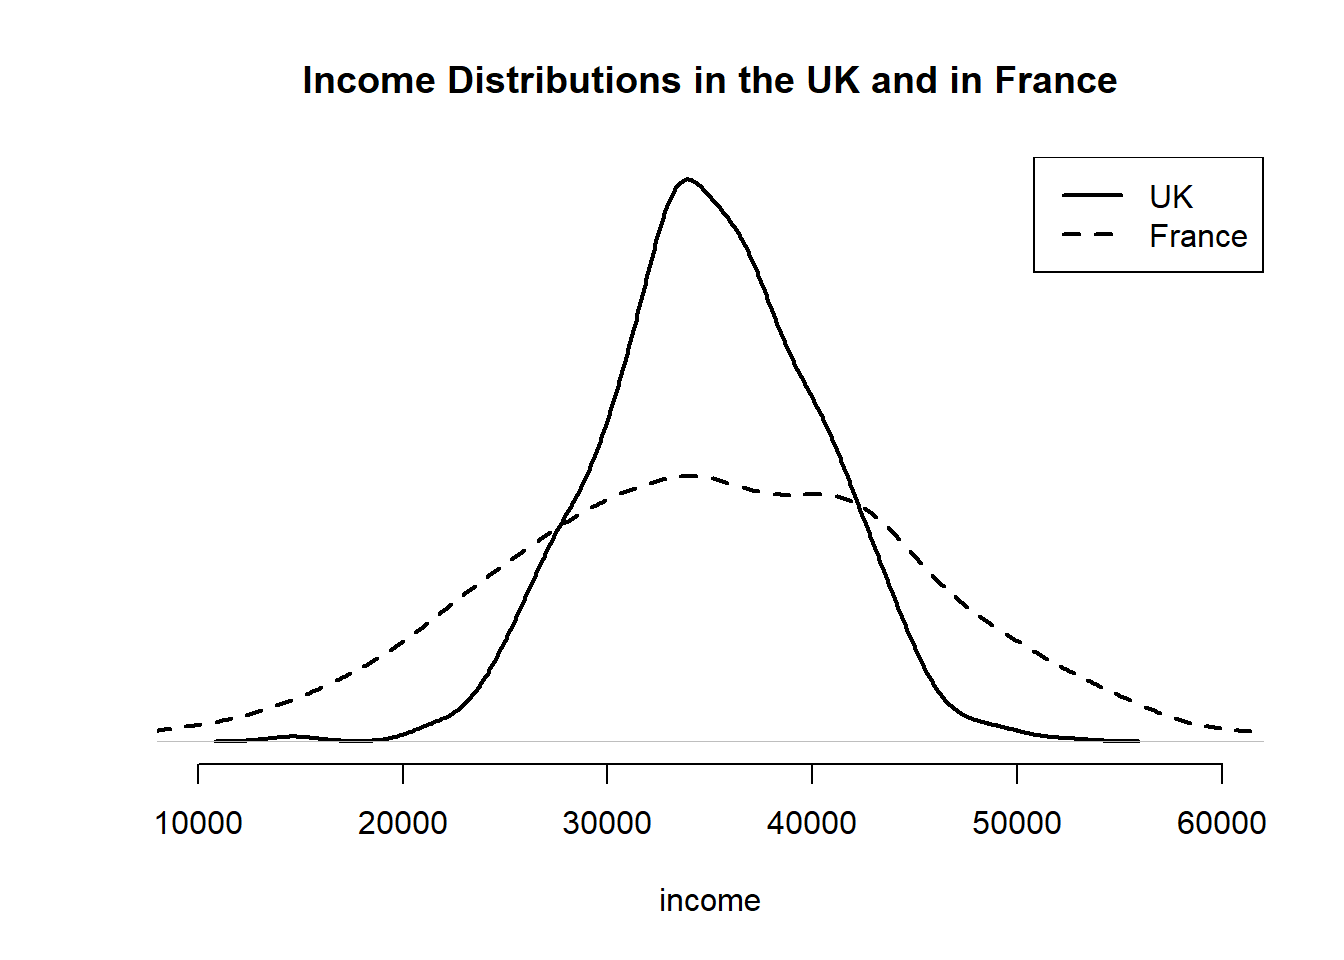
\includegraphics{statistics1_files/figure-latex/unnamed-chunk-26-1.pdf}

The variance gives us an idea about the variability of data. The formula
for the variance in the population is
\[ \frac{\sum_{i=1}^n(x_i - \mu_x)^2}{n}\]

The formula for the variance in a sample adjusts for sampling
variability, i.e., uncertainty about how well our sample reflects the
population by subtracting 1 in the denominator. Subtracting 1 will have
next to no effect if n is large but the effect increases the smaller n.
The smaller n, the larger the sample variance. The intuition is, that in
smaller samples, we are less certain that our sample reflects the
population. We, therefore, adjust variability of the data upwards. The
formula is

\[ \frac{\sum_{i=1}^n(x_i - \bar{x})^2}{n-1}\]

Notice the different notation for the mean in the two formulas. We write
\(\mu_x\) for the mean of x in the population and \(\bar{x}\) for the
mean of x in the sample. Notation is, however, unfortunately not always
consistent.

Take a minute to think your way through the formula. There are 4 setps:
(1), In the numerator, we subtract the mean of x from some realisation
of x. (2), We square the deviations from the mean because we want
positive numbers only. (3) We sum the squared deviations. (4) We divide
the sum by \((n-1)\). Below we show this for the homework example. In
the last row, we add a 5th step. We take the square root in order to
return to the orginial units of the homework grades.

\begin{longtable}[]{@{}llll@{}}
\toprule
Obs & Var & Dev. from mean & Squared dev. from mean\tabularnewline
\midrule
\endhead
i & grade & \(x_i-\bar{x}\) & \((x_i-\bar{x})^2\)\tabularnewline
1 & 80 & -3.9090909 & 15.2809917\tabularnewline
2 & 90 & 6.0909091 & 37.0991736\tabularnewline
3 & 85 & 1.0909091 & 1.1900826\tabularnewline
4 & 71 & -12.9090909 & 166.6446281\tabularnewline
5 & 69 & -14.9090909 & 222.2809917\tabularnewline
6 & 85 & 1.0909091 & 1.1900826\tabularnewline
7 & 83 & -0.9090909 & 0.8264463\tabularnewline
8 & 88 & 4.0909091 & 16.7355372\tabularnewline
9 & 99 & 15.0909091 & 227.7355372\tabularnewline
10 & 81 & -2.9090909 & 8.4628099\tabularnewline
11 & 92 & 8.0909091 & 65.4628099\tabularnewline
\(\sum_{i=1}^n\) & & & 762.9090909\tabularnewline
\(\div n-1\) & & & 76.2909091\tabularnewline
\(\sqrt{}\) & & & 8.7344667\tabularnewline
\bottomrule
\end{longtable}

Our first grade (80) is below the mean (83.9090909). The sum is, thus,
negative. Our second grade (90) is above the mean, so that the sum is
positive. Both are deviations from the mean (think of them as
distances). Our sum shall reflect the total sum of distances and
distances must be positive. Hence, we square the distances from the
mean. Having done this for all eleven observations, we sum the squared
distances. Dividing by 10 (with the sample adjustment), gives us the
average squared deviation. This is the variance. The units of the
variance---squared deviations---are somewhat awkward. We return to this
in a moment.

We take the variance in R by using the
\href{http://bit.ly/R_var}{\texttt{var()}} function. By default
\texttt{var()} takes the sample variance.

\begin{Shaded}
\begin{Highlighting}[]
\KeywordTok{var}\NormalTok{(hw.grades)}
\end{Highlighting}
\end{Shaded}

\begin{verbatim}
[1] 76.29091
\end{verbatim}

The average squared difference form our mean grade is 76.2909091. But
what does that mean? We would like to get rid of the square in our
units. That's what the standard deviation does. The standard deviation
is the square root over the variance.

\[ \sqrt{\frac{\sum_{i=1}^n(x_i - \bar{x})^2}{n-1}}\]

We get the average deviation from our mean grade (83.9090909) with the
\href{http://bit.ly/R_sd}{\texttt{sd()}} function.

\begin{Shaded}
\begin{Highlighting}[]
\KeywordTok{sd}\NormalTok{(hw.grades)}
\end{Highlighting}
\end{Shaded}

\begin{verbatim}
[1] 8.734467
\end{verbatim}

The standard deviation is much more intuitive than the variance because
its units are the same as the units of the variable we are interested
in. ``Why teach us about this awful variance then'', you ask.
Mathematically, we have to compute the variance before getting the
standard deviation. We recommend that you use the standard deviation to
describe the variability of your continuous data.

\subsubsection{Range and interquartile
range}\label{range-and-interquartile-range}

The proper measure of dispersion of an ordinal variable is the range or
the interquartile range. The interquartile range is usually the
preferred measure because the range is strongly affected by outlying
cases.

Let's take the range first. We get back to our education example. In R,
we use the \href{http://bit.ly/R_range}{\texttt{range()}} function to
compute the range.

\begin{Shaded}
\begin{Highlighting}[]
\KeywordTok{range}\NormalTok{(edu)}
\end{Highlighting}
\end{Shaded}

\begin{verbatim}
[1] 0 5
\end{verbatim}

Our data ranges from no education all the way to those with a doctorate.
However, no education is not a common value. Only one person in our
sample did not have any education. The interquartile range is the range
from the 25th to the 75th percentiles, i.e., it contains the central 50
percent of the distribution.

The 25th percentile is the value of education that 25 percent or fewer
people have (when we order education from lowest to highest). We use the
\href{http://bit.ly/R_quantile}{\texttt{quantile()}} function in R to
get percentiles. The function takes two arguments: \texttt{x} is the
data vector and \texttt{probs} is the percentile.

\begin{Shaded}
\begin{Highlighting}[]
\KeywordTok{quantile}\NormalTok{(edu, }\FloatTok{0.25}\NormalTok{) }\CommentTok{# 25th percentile}
\end{Highlighting}
\end{Shaded}

\begin{verbatim}
25% 
  2 
\end{verbatim}

\begin{Shaded}
\begin{Highlighting}[]
\KeywordTok{quantile}\NormalTok{(edu, }\FloatTok{0.75}\NormalTok{) }\CommentTok{# 75th percentile}
\end{Highlighting}
\end{Shaded}

\begin{verbatim}
75% 
  3 
\end{verbatim}

Therefore, the interquartile range is from 2, secondary school to 3,
undergraduate degree.

\subsubsection{Proportion in each
category}\label{proportion-in-each-category}

To describe the distribution of our nominal variable, support for
remaining in the European Union, we use the proportions in each
category.

Recall, that we looked at the frequency table to determine the mode:

\begin{Shaded}
\begin{Highlighting}[]
\KeywordTok{table}\NormalTok{(stay)}
\end{Highlighting}
\end{Shaded}

\begin{verbatim}
stay
  0   1 
509 491 
\end{verbatim}

To get the proportions in each category, we divide the values in the
table, i.e., 509 and 491, by the sum of the table, i.e., 1000.

\begin{Shaded}
\begin{Highlighting}[]
\KeywordTok{table}\NormalTok{(stay) }\OperatorTok{/}\StringTok{ }\KeywordTok{sum}\NormalTok{(}\KeywordTok{table}\NormalTok{(stay))}
\end{Highlighting}
\end{Shaded}

\begin{verbatim}
stay
    0     1 
0.509 0.491 
\end{verbatim}

\subsection{Exercises}\label{exercises}

\begin{enumerate}
\def\labelenumi{\arabic{enumi}.}
\tightlist
\item
  Create a script and call it assignment01. Save your script.
\item
  Download this
  \href{https://www.rstudio.com/wp-content/uploads/2016/06/r-cheat-sheet.pdf}{cheat-sheet}
  and go over it. You won't understand most of it right a away. But it
  will become a useful resource. Look at it often.
\item
  Calculate the square root of 1369 using the \texttt{sqrt()} function.
\item
  Square the number 13 using the \texttt{\^{}} operator.
\item
  What is the result of summing all numbers from 1 to 100?
\end{enumerate}

We take a sample of yearly income in Berlin. The values that we got are:
19395, 22698, 40587, 25705, 26292, 42150, 29609, 12349, 18131, 20543,
37240, 28598, 29007, 26106, 19441, 42869, 29978, 5333, 32013, 20272,
14321, 22820, 14739, 17711, 18749.

\begin{enumerate}
\def\labelenumi{\arabic{enumi}.}
\tightlist
\item
  Create the variable \texttt{income} with the values form our Berlin
  sample in R.
\item
  Describe Berlin income using the appropriate measures of central
  tendency and dispersion.
\item
  Compute the average deviation without using the \texttt{sd()}
  function.
\end{enumerate}

Take a look at the Sunday Question (who would you vote for if the
general election were next Sunday?) by following this link
\href{https://www.wahlrecht.de/umfragen/}{Sunday Question Germany}. You
should be able to translate the website into English by right clicking
in your browser and clicking ``Translate to English.''

\begin{enumerate}
\def\labelenumi{\arabic{enumi}.}
\tightlist
\item
  What is the level of measurement of the variable in the Sunday
  Question?
\item
  Take the most recent poll and describe what you see in terms of
  central tendency and dispersion.
\item
  Save your script, which should now include the answers to all the
  exercises.
\item
  Source your script, i.e.~run the entire script without error message.
  Clean your script if you get error messages.
\end{enumerate}


\end{document}
